% arara: xelatex: {shell: true}
% arara: biber
% arara: makeglossaries
% arara: xelatex: {shell: true}
% arara: xelatex: {shell: true}
\documentclass[letterpaper,10pt]{article}
\usepackage[margin=1in]{geometry}
\usepackage{newfloat}
\usepackage{hyperref}
\usepackage{graphicx}
\usepackage[justification=centering,font=small,labelfont=bf]{caption}
\usepackage{fancyhdr}
\usepackage{parskip}
\usepackage{fontspec}
\usepackage[toc,nonumberlist,xindy]{glossaries}
\usepackage{relsize}
\setmonofont{Inconsolata}[Scale=MatchLowercase]
\defaultfontfeatures{Ligatures=TeX}
\usepackage{xeCJK}
\usepackage{xcolor}
\usepackage[titletoc,title]{appendix}
\usepackage{wrapfig}
\usepackage{minted}
\usepackage{csquotes}
\usepackage{polyglossia}
\setmainlanguage{english}
\setotherlanguage{hebrew}
\newfontfamily\hebrewfont[Scale=0.8,Script=Hebrew]{Frank Ruehl CLM}
\definecolor{dsscawpurp}{HTML}{b079b0}
\definecolor{dsscawpurpcap}{HTML}{6c286c}
\usepackage[font={color=dsscawpurpcap},labelfont={sc}]{caption}
\usepackage[backend=biber,
date=iso,
seconds=true,
style=numeric,
bibencoding=utf8,
]{biblatex}

\addbibresource{\jobname.bib}
\usemintedstyle{friendly}
\newenvironment{denseitemize}{
  \begin{itemize}
      \setlength{\itemsep}{0pt}
}{
  \end{itemize}
}
% An attractive 'C++'
\newcommand\CC{C\nolinebreak\hspace{-.05em}\raisebox{.4ex}{\relsize{-3}{\textbf{+}}}\nolinebreak\hspace{-.10em}\raisebox{.4ex}{\relsize{-3}{\textbf{+}}}\hspace{.2em}}

\pagestyle{fancy}
\rhead{
  
\includegraphics[height=\fontcharht\font`\D,keepaspectratio=true]{../dsscaw-hdr.pdf}
  \textcolor{dsscawpurp}{DSSCAW Technical Report \#004}
}

\title{Hacking the Planet! with Notcurses:\\
A Guide to TUIs and Character Graphics\thanks{
 \href{https://www.dsscaw.com/}{Dirty South Supercomputing of Atlanta, GA. Free documentation under the Apache 2.0 License.}
}\\
}
\author{Nick Black, Consulting Scientist\\
\texttt{nickblack@linux.com}
}


\makeglossaries
\setglossarypreamble{When possible, I have followed the definitions of
  RFC 2978\cite{rfc2978} and the Glossary of Unicode Terms\cite{unicodeglossary}.}
\loadglsentries{glossary}

%%%%%%%%%%%%%%%%%%%%%%%%%%%%%%%%%%%%%%%%%%%%%%%%%%%%%%%%%%%%%%%%%%%%%%%%
\begin{document}
%%%%%%%%%%%%%%%%%%%%%%%%%%%%%%%%%%%%%%%%%%%%%%%%%%%%%%%%%%%%%%%%%%%%%%%%
\date{Feb 14, 2020}
\maketitle
\thispagestyle{fancy}
\date{}
\vspace{1in}
\begin{center}
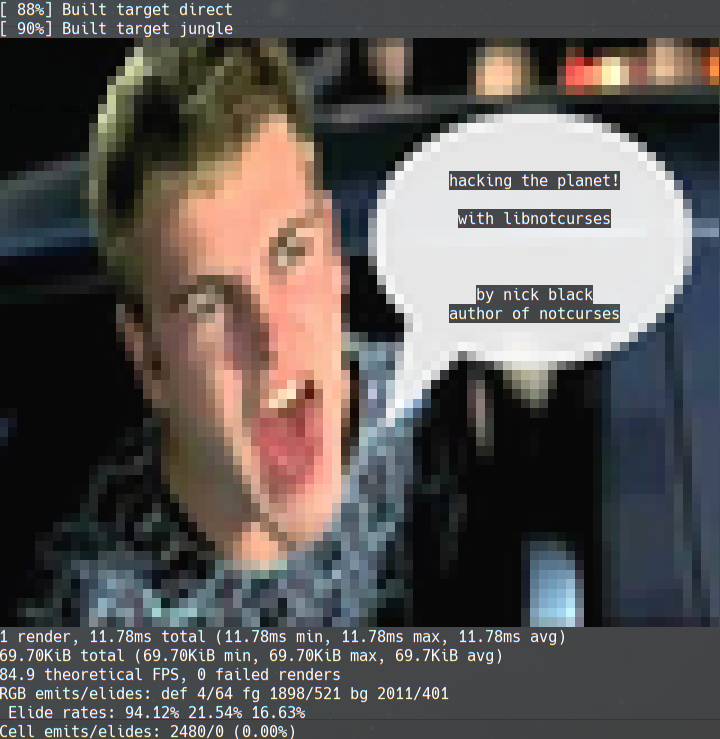
\includegraphics[width=.75\linewidth]{htp-with-notcurses.png}
\end{center}
%%%%%%%%%%%%%%%%%%%%%%%%%%%%%%%%%%%%%%%%%%%%%%%%%%%%%%%%%%%%%%%%%%%%%%%%

\clearpage

\tableofcontents

\clearpage

\section{Introduction}

I implemented Notcurses in the winter of 2019 after having a few patches
rejected from NCURSES. The first commit was pushed 2019-11-16. I started
writing this manuscript 2020-02-12, following the 1.1.8 release. It proved to
be seductive as hell, and it was only with difficulty that I tore myself away
following three months of hard work. By that time, Notcurses subsumed large
chunks of NCURSES, adding a great deal more. The project had three
major goals:

\begin{denseitemize}
\item to provide NCURSES-like functionality with 24-bit color, safety in the
    presence of multithreading, and full Unicode support,
\item to reduce the amount of boilerplate code necessary for the UIs of my
    TUI applications, including \textit{growlight} and \textit{omphalos}, and
\item to portably facilitate the most vivid character graphics possible.
\end{denseitemize}

Many people asked how such a thing was useful. My usual response was that
numerous devices don't present a bitmap interface, that X11 GUIs run remotely
over SSH are effectively unusable, that plenty of machines don't have a GUI
environment installed, and that Sixel isn't well-supported across different
terminal emulators. It seems impossible in an age of gigatransistor graphics
cards, but the text environment still presents perceivably less latency
than most GUI toolkits. That I was able to remove thousands of lines
of NCURSES code from my applications was a nice side benefit.

In truth, the main reasons were that it was fun, and I wanted to see how far
I could push it.

As I write this, Notcurses is present in Arch's AUR, and is awaiting promotion
into the Debian Incoming queue. Written as a C core, it enjoys \CC, Python, and
Rust wrappers. I have submitted it as a backend to NEStopia and RetroArch, and
intend to integrate it into Mesa as an OpenGL backend. So long as one can live
with the limited resolution available when a screen is divided into rectangular
cells, it can handle any graphics thrown at it. I hope to see it displace
NCURSES as the go-to character graphics library for new applications (there is
little value in porting existing applications to Notcurses, since an unchanged
application wouldn't take advantage of its advanced features).

While the X/OSI Curses specification is unlikely to ever go away (nor should
it, as a lowest-common-denominator interface to devices Notcurses is unlikely
to ever support), I believe Notcurses to present a superior API and
implementation for modern TUI applications.

The console ain't dead! Hack on, hax0rs.

\vspace{.5in}

\begin{flushright}
  \textit{---February 2020, Atlanta}
\end{flushright}

\vspace{1in}

\begin{center}
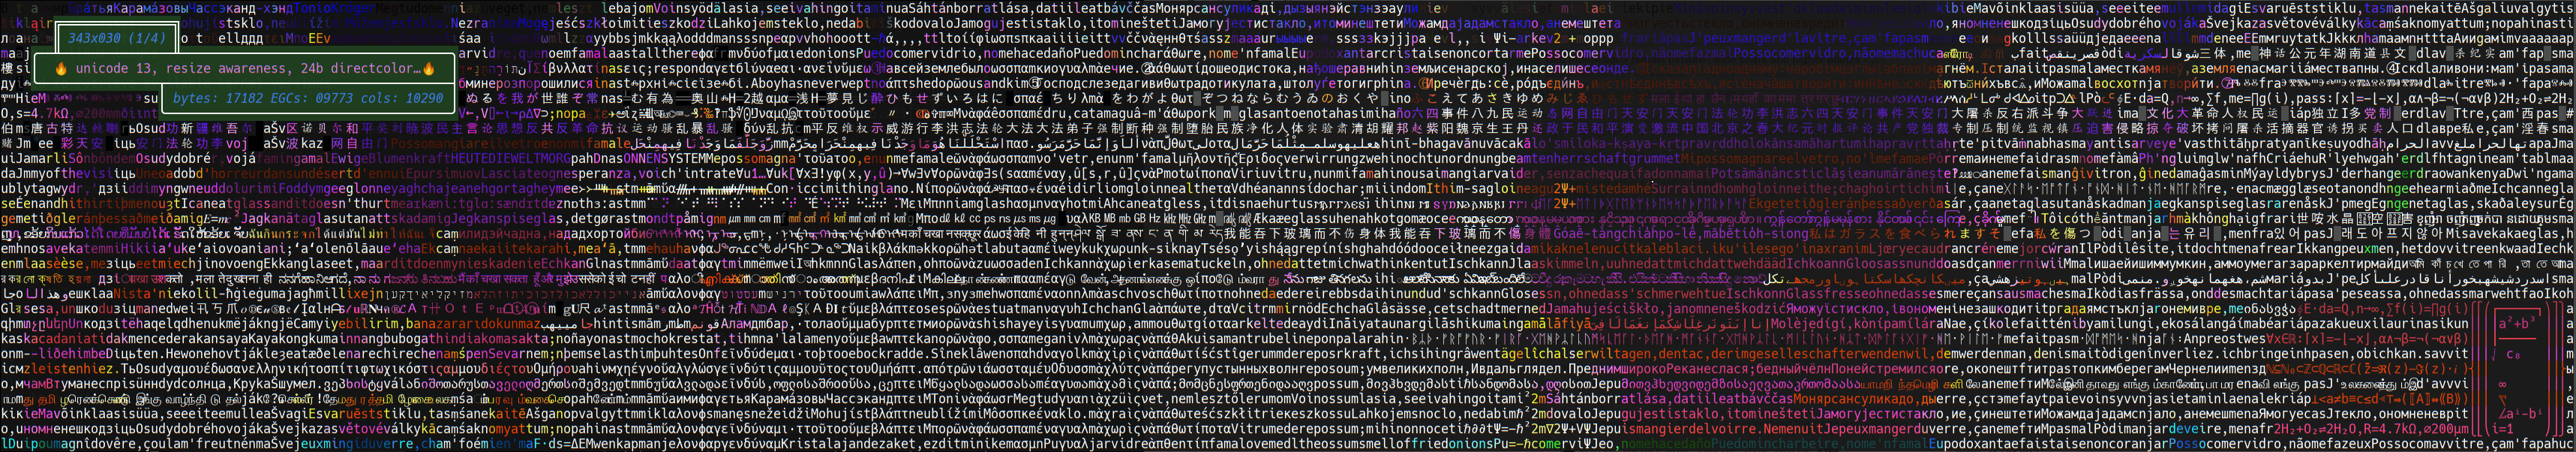
\includegraphics[width=1\linewidth]{media/widechars.png}
\end{center}

\newpage
%%%%%%%%%%%%%%%%%%%%%%%%%%%%%%%%%%%%%%%%%%%%%%%%%%%%%%%%%%%%%%%%%%%%%%%%

\section{Using direct mode with standard I\/O}

Many tools don't intend to be full-screen TUI applications, but instead
implement that purest of UNIX interfaces: newline-delimited text, oblivious
to screen geometry, capable of being fed as input to other, similar programs.
For such tools, the full Notcurses capabilities are neither necessary nor
desirable. These programs are typically non-interactive: humans might peruse
their outputs and prepare their inputs, but they effectively run as a batch
task.

 Such tools might still want to colorize and otherwise style their output, at
least when being output to a terminal. This can be accomplished using the
\texttt{ncdirect} subset of Notcurses, and is known as \textit{direct mode}. Direct
mode functionality should not usually be mixed with other Notcurses calls.
Unlike full Notcurses, there is no explicit rendering step in direct mode, and
it is intended to be mixed among other use of standard I/O. Essentially, direct
mode ``styles your \texttt{printf()}s.'' Similarly to full Notcurses, direct mode
requires a valid and correct terminfo database entry, supplied via either the
\texttt{termtype} parameter to \texttt{notcurses\_directmode()} or the \texttt{TERM} environment
variable. It does \textit{not}, however, require any particular encoding nor
even a call to \texttt{setlocale()} (full Notcurses requires a properly-configured
ASCII or UTF-8 locale).

Enter direct mode via a call to \texttt{notcurses\_directmode()} with a successful
return of a non-\texttt{NULL} pointer to \texttt{struct ncdirect}:

\begin{listing}[ht]
\begin{minted}{C}
// Initialize a direct-mode notcurses context on the connected terminal at 'fp'.
// 'fp' must be a tty. You'll usually want stdout. Direct mode supportes a
// limited subset of notcurses routines which directly affect 'fp', and neither
// supports nor requires notcurses_render(). This can be used to add color and
// styling to text in the standard output paradigm. Returns NULL on error,
// including any failure initializing terminfo.
struct ncdirect* notcurses_directmode(const char* termtype, FILE* fp);
\end{minted}
\end{listing}

It is typical to invoke this function as \texttt{notcurses\_directmode(NULL, stdout)}.
In this case, the terminal type must be present in the \texttt{TERM} environment
variable (this should have been done by the terminal). The buffering and
blocking status of \texttt{fp} will not be changed. \texttt{NULL} is returned for any number
of possible errors. Otherwise, the \texttt{struct ncdirect} is ready to go, and should
be cleaned up with \texttt{ncdirect\_stop()}:

\begin{listing}[ht]
\begin{minted}{C}
// Release 'nc' and any associated resources. 0 on success, non-0 on failure.
int ncdirect_stop(struct ncdirect* nc);
\end{minted}
\end{listing}

Between these two calls, inject stylizing control codes into the \texttt{FILE*} with
the following API:

\begin{listing}[ht]
\begin{minted}{C}
int ncdirect_bg_rgb8(struct ncdirect* n, unsigned r, unsigned g, unsigned b);
int ncdirect_fg_rgb8(struct ncdirect* n, unsigned r, unsigned g, unsigned b);
int ncdirect_fg(struct ncdirect* n, unsigned rgb);
int ncdirect_bg(struct ncdirect* n, unsigned rgb);
int ncdirect_fg_default(struct ncdirect* n);
int ncdirect_bg_default(struct ncdirect* n);
int ncdirect_styles_set(struct ncdirect* n, unsigned stylebits);
int ncdirect_styles_on(struct ncdirect* n, unsigned stylebits);
int ncdirect_styles_off(struct ncdirect* n, unsigned stylebits);
int ncdirect_clear(struct ncdirect* n);
\end{minted}
\end{listing}

While direct mode does not offer any means for moving the cursor in
two-dimensional space, it does provide helpers for determining the terminal
geometry:

%\begin{listing}[ht]
\begin{minted}{C}
int ncdirect_dim_x(const struct ncdirect* nc);
int ncdirect_dim_y(const struct ncdirect* nc);
\end{minted}
%\end{listing}

\subsection{Example: presenting \textit{\textcolor{blue}{House} of Leaves}}

Mark Z. Danielewski's experimental 2000 novel \textit{\textcolor{blue}{House} of Leaves}\cite{danielewski2000house} prints each
instance of the word \textcolor{blue}{house} in blue, even when it is a subword:

\begin{figure}[!htbp]
\centering 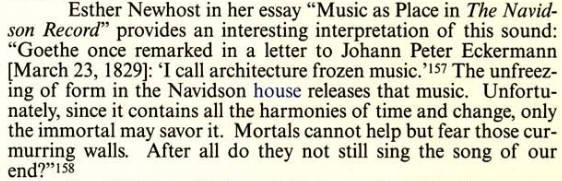
\includegraphics[width=.5\linewidth]{house-blue.png}
\caption{An excerpt from page 123 of \textit{\textcolor{blue}{House} of Leaves}.}
\label{fig:houseofleaves}
\end{figure}

We can easily write code to reproduce this effect for standard input and output.
The following works as expected (see Figure~\ref{fig:houseout}):

\begin{listing}[!htbp]
\inputminted[fontsize=\scriptsize]{C}{code/hol-formatter.c}
\caption{\texttt{hol-formatter.c}}
\end{listing}

There are a few things worth noting about the code above. First, observe how
much of the logic is devoted to checking and propagating errors! Perhaps
contrary to common expectation, reliable code--especially when that code's
primary effect is to write to stdout--generally needs to check the results of
e.g. \texttt{printf()} (what happens if we're redirected to a file, and
the disk is full?). A language making use of exceptions would reduce if not
eliminate this nonsense.

\begin{figure}[!htbp]
\centering 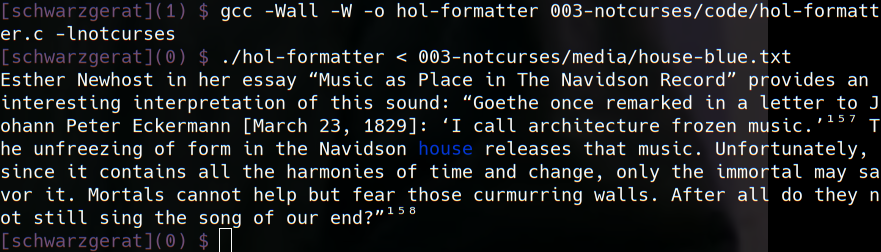
\includegraphics[width=.75\linewidth]{hol-formatted.png}
\caption{\texttt{hol-formatter} as run on our input. We use \texttt{tesseract} for OCR, with pleasantly solid results.}
\label{fig:houseout}
\end{figure}

We don't switch from blue to some random color, because we don't know the
background color of the terminal. Hard to believe as it is, some people don't
favor a dark terminal background. If the terminal background was white, and we
had just used e.g. \texttt{ncdirect\_fg(n, 0xffffff)}, text following
``\textcolor{blue}{house}'' would be invisible.

One might observe that a user with a blue background will have invisible
``\textcolor{blue}{house}'' text. This is true, and there's no great solution
to it. It is not generally possible to discover the RGB values of the default
colors. I suppose all one can do is rest easy, serene in the belief that people
with chromatic backgrounds deserve whatever happens to them.

\subsection{Example: colorizing a dumb game}

Imagine we've written the following guessing game:

\begin{listing}[!htbp]
\inputminted[fontsize=\scriptsize]{C}{code/hilostdio.c}
\caption{\texttt{hilostdio.c}}
\end{listing}

The correct approach is binary search, and for an $N$-bit \texttt{long}, we expect to
guess the number in no more than $N$ tries. Let's color the output to indicate how
bad of a guess was offered. We'll use red for low guesses, blue for high
guesses, and break the 256 shades of each (assuming the other two components
to be fixed) uniformly across the $N$ levels of logarithmic
distance\footnote{This would be a good place to employ \gls{gamma correction}.}.
If we wanted to do this without direct use of RGB color, we'd either need
accept fewer shades, or be forced to reprogram the palette.

\begin{listing}[!htbp]
\begin{minted}[fontsize=\scriptsize]{C}
    if(!(r |= (ncdirect_fg_default(n)))){
          ...
          int offoom = labs(__builtin_clzl(guess) - __builtin_clzl(secret));
          if(guess > secret){
            r |= ncdirect_fg_rgb8(n, 0x40, 0x80, offoom * 6);
          }else if(guess < secret){
            r |= ncdirect_fg_rgb8(n, offoom * 6, 0x80, 0x40);
          ...
\end{minted}
\caption{Insertions into \texttt{hilostdio.c} yielding \texttt{hilodirect.c}.}
\end{listing}

Stepping through the orders of magnitude, we get the expected gradient. Were
we to actually play, the response would converge to a balanced, strong green
as we approached the correct answer.

\begin{figure}[!htbp]
\centering 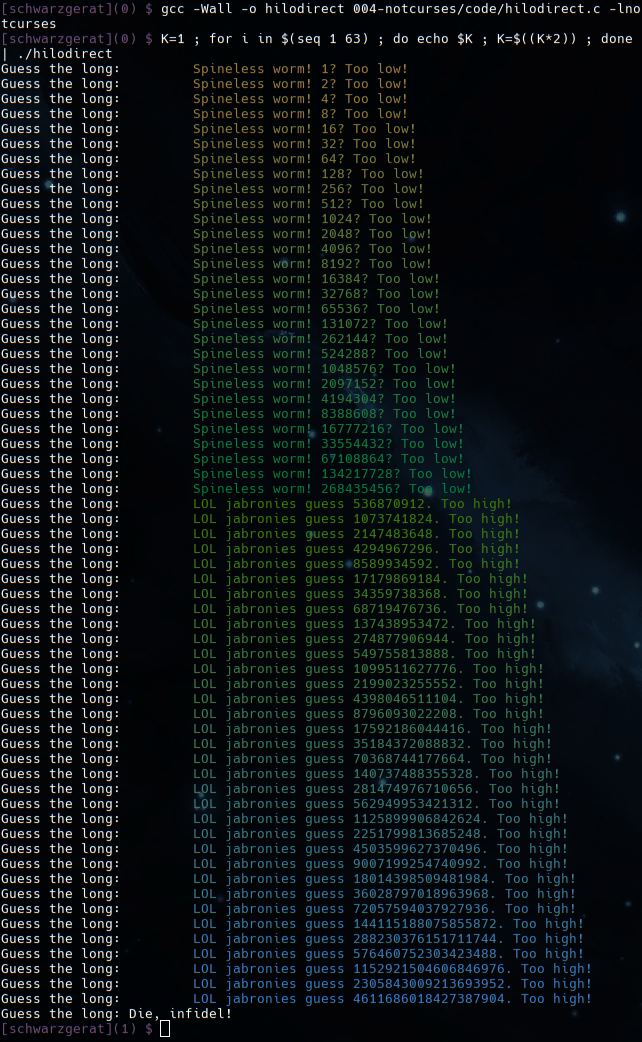
\includegraphics[width=.75\linewidth]{media/hilodirect.png}
\caption{Colorized output from \texttt{hilodirect.c}.}
\end{figure}
\newpage

%%%%%%%%%%%%%%%%%%%%%%%%%%%%%%%%%%%%%%%%%%%%%%%%%%%%%%%%%%%%%%%%%%%%%%%%
\section{Using fullscreen mode}
From this chapter forward, we will be using the fullscreen mode of Notcurses,
opening up all of its capabilities. This comes at a cost: while fullscreen mode
is being used, it is not safe to use standard I/O in conjunction with the
terminal controlled by Notcurses. Doing so is likely to (at a minimum) corrupt
the screen. If \texttt{stdout} and \texttt{stderr} are attached to the same
terminal (as they usually are in an interactive session), and \texttt{stdout}
is provided to Notcurses, output to \texttt{stderr} will corrupt the display
just as thoroughly as output to \texttt{stdout}. If your fullscreen Notcurses
program intends to log to \texttt{stderr}, you should first ensure that that
it has been redirected or is otherwise going somewhere different than
\texttt{stdout}. Note that simply rerendering the output will \textit{not}
necessarily clean up corruption, even following \texttt{ncplane\_erase()}
operations, since Notcurses optimizes its rendering based on its concept of the
screen. A call to \texttt{notcurses\_refresh()} will be necessary to sync the
the physical screen to Notcurses's concept thereof.

It is possible for the screen to be corrupted by external agents. For this
reason, Ctrl+L is by tradition bound to screen redrawing. You should hook this
input up to \texttt{notcurses\_refresh()} unless you have good reasons not to
do so (this is not default behavior of Notcurses only because Notcurses does
not itself read input). It is sadly not possible for such corruption to be
efficiently and generally detected.

It is possible for the attached terminal to be resized, especially (but not
only) for terminal emulators in GUI windowing environments\footnote{This could
also happen when refitting a \texttt{screen} or \texttt{tmux} session.
Even on the Linux or FreeBSD console, this can happen due to a change in video
resolution.}. Notcurses can detect such events, and synthesizes
\texttt{NCKEY\_RESIZE} inputs in response to them. If the screen shrinks, the
excess data relative to the constant origin will no longer be displayed (i.e.
the material in the upper left will be retained). If the screen is enlarged,
any data uncovered will be displayed, and the new area will otherwise be empty.
Some widgets can intelligently resize themselves in the face of screen
geometry changes (see Chapter~\ref{section:uiwidgets}).

Notcurses prepares a given terminal for fullscreen mode in the
\texttt{notcurses\_init} function:

\begin{listing}[!htbp]
\begin{minted}{C}
// Initialize a notcurses context on the connected terminal at 'fp'. 'fp' must
// be a tty. You'll usually want stdout. Returns NULL on error, including any
// failure initializing terminfo.
struct notcurses* notcurses_init(const notcurses_options* opts, FILE* fp);

// Destroy a notcurses instance, restoring the terminal to its original state.
int notcurses_stop(struct notcurses* nc);
\end{minted}
\end{listing}

Before calling \texttt{notcurses\_init()} (and usually as one of the first lines
of the program) it is necessary to set the current locale via the standard
library function \texttt{setlocale()}. A coverage of ANSI/ISO C locales is beyond
the scope of this text, but it is usually sufficient to call
\texttt{setlocale(LC\_ALL, "")}, relying on the user's configured \texttt{LANG}
environment variable. Notcurses only supports those locales using
US-ASCII or UTF-8 encodings (see Chapter~\ref{section:unicode} for more
information on character encodings), and its capabilities on US-ASCII
are \textit{severely} constrained. \texttt{notcurses\_init()} will return an
error for any other encoding (see Figure~\ref{fig:encodingfail}).

\begin{figure}[!htbp]
\centering 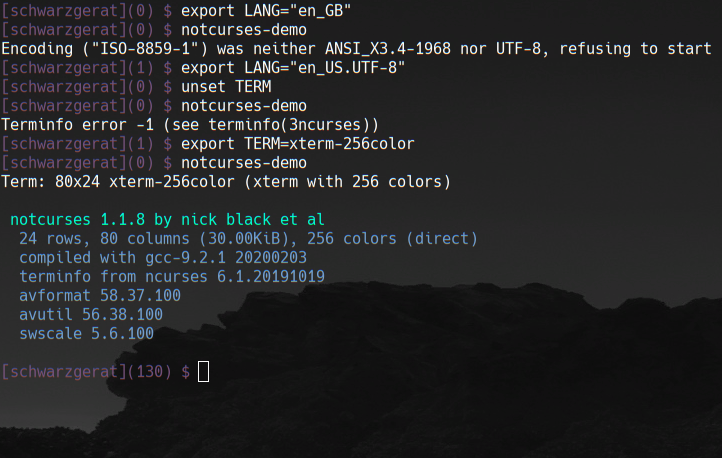
\includegraphics[width=.7\linewidth]{media/notcurses-init-fails.png}
\caption{Notcurses refusing to start due to an unsupported character encoding.}
\label{fig:encodingfail}
\end{figure}

By default (assuming the \texttt{enter\_ca\_mode} terminfo capability is expressed),
Notcurses attempts to enter the ``\gls{smcup}''. Using the alternate screen
implies:
\begin{denseitemize}
\item{The screen will be cleared upon entry,}
\item{Output will not be appended to the scrollback buffer, and}
\item{On exit, output will be cleared.}
\end{denseitemize}
Whether or not the original screen contents are restored is terminal-dependent
(if the \texttt{non\_rev\_rmcup} terminfo capability is defined, the original
contents will \textit{not} be restored). This can be useful, but some users
don't like it, so it's wise to expose this via a configuration option.
Disabling use of the alternate screen can be done via the
\texttt{notcurses\_options} field \texttt{inhibit\_alternate\_screen}.

Successful creation of a \texttt{struct notcurses} implies the existence of
a \texttt{struct ncplane}, the ``standard plane''\footnote{\texttt{ncplane}s,
discussed in depth in Chapter~\ref{ncplane}, are the fundamental drawing surfaces of Notcurses.}.
This standard plane cannot be destroyed without destroying the containing
Notcurses context, nor can it be moved or resized by the user. Its size always
matches Notcurses's conception of the terminal's screen size, and its origin
always corresponds precisely to the terminal's origin. Aside from these
restrictions, the standard plane is a drawable surface like any other
\texttt{ncplane}---it can be moved along the z-axis, written to with arbitrary
glyphs and styles, made transparent, etc.

Once you're done using a \texttt{struct notcurses}, it's important to destroy
it with \texttt{notcurses\_stop}, even if your process exits abnormally. By
default, Notcurses registers signal handlers for most fatal signals. These
handlers will call \texttt{notcurses\_stop()} and then pass the signal to the
orginal actions. You can disable this with the \texttt{no\_quit\_sighandlers}
field of \texttt{notcurses\_options}, but there aren't very many good reasons
to do so.

\subsection{The \texttt{notcurses\_options} structure}
The first parameter to \texttt{notcurses\_init} is a (possibly \texttt{NULL})
\texttt{notcurses\_options}. This structure has been defined such that the
default options are equivalent to a zero-initialized structure. Passing \texttt{NULL}
is thus equivalent to passing a zero-initialized \texttt{notcurses\_options}.
The fields therein include:
\begin{denseitemize}
\item{\texttt{const char* termtype}: The name of the terminfo database entry to
    use. If \texttt{NULL}, the value of the environment variable \texttt{TERM}
    is used. Failure to initialize the terminfo database will result in a
    \texttt{notcurses\_init()} failure.} A defined but invalid or suboptimal
    entry will result in garbage, missing output, poor performance, reduced
    colors, and unsightly weight gain.
\item{\texttt{bool inhibit\_alternate\_screen}: As noted above, this prevents
    Notcurses from making use of the alternate screen, even if the \texttt{enter\_ca\_mode}
    terminfo capability is defined. It's best to wire this up to a user-managed
    option. Not using the alternate screen can look weird upon return to the
    shell (see Figure~\ref{fig:altscreen}).

\begin{figure}[!htbp]
\centering 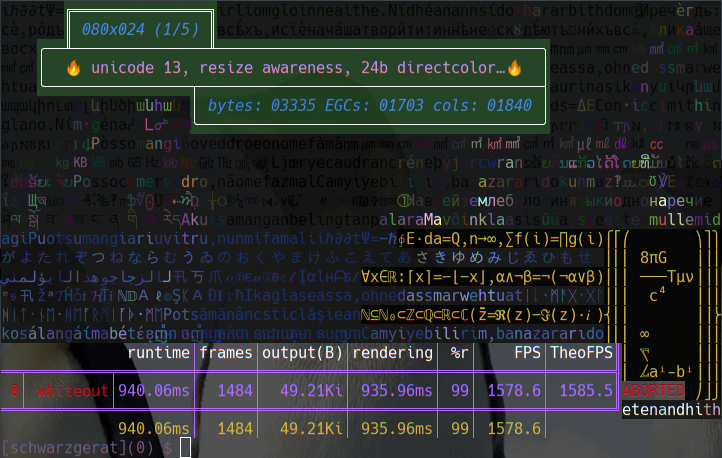
\includegraphics[width=.7\linewidth]{media/no-alternate-screen.png}
\caption{\texttt{notcurses-demo} can be invoked with \texttt{-k} to avoid
  using the alternate screen. Here, we see its output left on the screen as
  we return to our shell.}
\label{fig:altscreen}
\end{figure}
  }
\item{\texttt{bool retain\_cursor}: Notcurses hides the cursor by default.
    Set this to keep the cursor visible (the cursor can be turned on and off
    at runtime with \texttt{notcurses\_cursor\_enable()} and
    \texttt{notcurses\_cursor\_disable()}).}
\item{\texttt{bool suppress\_banner}: At startup, Notcurses emits some
    diagnostics and/or warnings, including version information and details
    about the current terminal. At shutdown, it prints performance statistics.
    These outputs \textit{do not} go to the alternate screen. Set this
    field to disable these outputs, but be aware that doing so might hide
    important warnings (see Figure~\ref{fig:banner}).

    \begin{figure}[!htbp]
      \centering 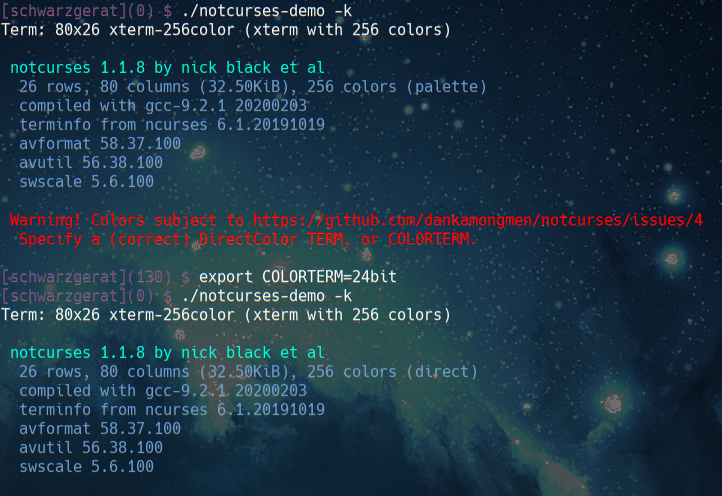
\includegraphics[width=.7\linewidth]{media/notcurses-banner.png}
      \caption{Initializing Notcurses without 24-bit color support will
        generate a warning, hopefully provoking your users to set it up.}
      \label{fig:banner}
    \end{figure}
}
\item{\texttt{bool no\_quit\_sighandlers}, \texttt{bool no\_winch\_sighandler}:
    As noted above, Notcurses by default registers signal actions for the normally fatal
    \texttt{SIGABRT}, \texttt{SIGINT}, \texttt{SIGQUIT}, and \texttt{SIGSEGV}.
    These handlers will call \texttt{notcurses\_stop} before propagating the
    signal to the original actions. This is usually desirable, as the screen
    will not otherwise be restored to its previous state. In addition, \texttt{SIGWINCH}
    is caught in order to generate \texttt{NCKEY\_RESIZE} inputs. If you
    disable these handlers, you'll almost certainly want to replace them with
    similar functionality.}
\item{\texttt{FILE* renderfp}: If not \texttt{NULL}, this designates a file
    handle open for writing. In addition to the terminal, each rendered scene
    will be written to this file. This is intended for debugging.}
\end{denseitemize}

\subsection{Functions on \texttt{notcurses} objects}

Output is not written to this top-level \texttt{struct notcurses}---that's
done with \texttt{ncplane}s---but there are a number of functions
available for these objects.

\begin{listing}[!htbp]
\begin{minted}{C}
// Get a reference to the standard plane (one matching our current idea of the
// terminal size) for this terminal. The standard plane always exists, and its
// origin is always at the uppermost, leftmost cell of the terminal.
struct ncplane* notcurses_stdplane(struct notcurses* nc);

// Create a new ncplane at the specified offset (relative to the standard plane)
// and the specified size. The number of rows and columns must both be positive.
// This plane is initially at the top of the z-buffer, as if ncplane_move_top()
// had been called on it. The void* 'opaque' can be retrieved (and reset) later.
struct ncplane* ncplane_new(struct notcurses* nc, int rows, int cols,
                            int yoff, int xoff, void* opaque);

// Return the topmost ncplane, of which there is always at least one.
struct ncplane* notcurses_top(struct notcurses* n);

// Destroy any ncplanes other than the stdplane.
void notcurses_drop_planes(struct notcurses* nc);
\end{minted}
\end{listing}

\begin{listing}[!htbp]
\begin{minted}{C}
// Make the physical screen match the virtual screen. Changes made to the
// virtual screen (i.e. most other calls) will not be visible until after a
// successful call to notcurses_render().
int notcurses_render(struct notcurses* nc);
\end{minted}
\end{listing}

\begin{listing}[!htbp]
\begin{minted}{C}
// See ppoll(2) for more detail. Provide a NULL 'ts' to block at length, a 'ts'
// of 0 for non-blocking operation, and otherwise a timespec to bound blocking.
// Signals in sigmask (less several we handle internally) will be atomically
// masked and unmasked per ppoll(2). It should generally contain all signals.
// Returns a single Unicode code point, or (char32_t)-1 on error. 'sigmask' may
// be NULL. Returns 0 on a timeout. If an event is processed, the return value
// is the 'id' field from that event. 'ni' may be NULL.
char32_t notcurses_getc(struct notcurses* n, const struct timespec* ts,
                        sigset_t* sigmask, ncinput* ni);

// 'ni' may be NULL if the caller is uninterested in event details. If no event
// is ready, returns 0.
static inline char32_t
notcurses_getc_nblock(struct notcurses* n, ncinput* ni){
  sigset_t sigmask;
  sigfillset(&sigmask);
  struct timespec ts = { .tv_sec = 0, .tv_nsec = 0 };
  return notcurses_getc(n, &ts, &sigmask, ni);
}

// 'ni' may be NULL if the caller is uninterested in event details. Blocks
// until an event is processed or a signal is received.
static inline char32_t
notcurses_getc_blocking(struct notcurses* n, ncinput* ni){
  sigset_t sigmask;
  sigemptyset(&sigmask);
  return notcurses_getc(n, NULL, &sigmask, ni);
}

// Enable the mouse in "button-event tracking" mode with focus detection and
// UTF8-style extended coordinates. On failure, -1 is returned. On success, 0
// is returned, and mouse events will be published to notcurses_getc().
int notcurses_mouse_enable(struct notcurses* n);

// Disable mouse events. Any events in the input queue can still be delivered.
int notcurses_mouse_disable(struct notcurses* n);
\end{minted}
\end{listing}

\begin{listing}[!htbp]
\begin{minted}{C}
int notcurses_resize(struct notcurses* n, int* restrict y, int* restrict x);

// Refresh the physical screen to match what was last rendered (i.e., without
// reflecting any changes since the last call to notcurses_render()). This is
// primarily useful if the screen is externally corrupted.
int notcurses_refresh(struct notcurses* n);
\end{minted}
\end{listing}

Finally, before ever creating a \texttt{notcurses}, we can call
\texttt{notcurses\_version} to get a human-readable string describing the
loaded library's version.

\newpage

%%%%%%%%%%%%%%%%%%%%%%%%%%%%%%%%%%%%%%%%%%%%%%%%%%%%%%%%%%%%%%%%%%%%%%%%
\section{A simple notcurses render\slash event loop}
I'm not typically a fan of example-based instruction, preferring to build things
up from formal axioms. Following chapters will effect such an approach. First,
however, let's work a semi-substantial example covering a varied set of
notcurses routines. We're going to create seven planes, one for each time
of tetromino, and map an image file to the background. We'll add mouse and
keyboard support for switching between the pieces, rotating them, and sliding
them around the screen. Finally, we'll implement collision detection, and
fluid handling of screen resizings. In the course of doing so, you'll learn
several important notcurses techniques:

\begin{denseitemize}
\item{Drawing and rotating these tetrominos will involve colors, gradients, and
      transparencies. The former are fundamental drawing tools. The latter is
      all one needs for sprites.}
\item{Mapping the background will involve image decoding, scaling, and blitting.}
\item{We'll cover most of what's to be known regarding input.}
\end{denseitemize}

This example will be picked up and further developed in the Tetris case study
of §~\ref{section:casestudy}.

\begin{figure}[!htbp]
\centering 
\includegraphics[width=.5\linewidth]{media/tetrominos.png}
\caption{Piping hot tetrominos, fresh from \textit{Spiritus Mundi}.}
\label{fig:tetrominos}
\end{figure}

\subsection{Example: moving a tetromino with keyboard+mouse}
\textbf{FIXME FIXME FIXME}

\newpage

%%%%%%%%%%%%%%%%%%%%%%%%%%%%%%%%%%%%%%%%%%%%%%%%%%%%%%%%%%%%%%%%%%%%%%%%

\section{Character encodings and glyphs}
\label{section:unicode}
Before continuing any further, it would behoove us to become familiar with our
core building blocks---character sets and their rasterization. Even if we were
to shrink the character cell to a single pixel, we'd still need write one or
another character into it, and emit a control code to stylize it\footnote{I've
seen this idea bandied about as if it's a serious suggestion. Besides the fact
that it won't work in a console, escapes are \textit{far} less efficient than
canvases or OpenGL display lists; if your plan involves using ANSI escape
sequences to drive a 1920x1080 display via roughly two million 1x1 character
cells, you're not going to space today, or maybe ever\cite{upgoerfive}.}.
\subsection{The Universal Character Set}
\subsection{UTF-8}

\begin{center}
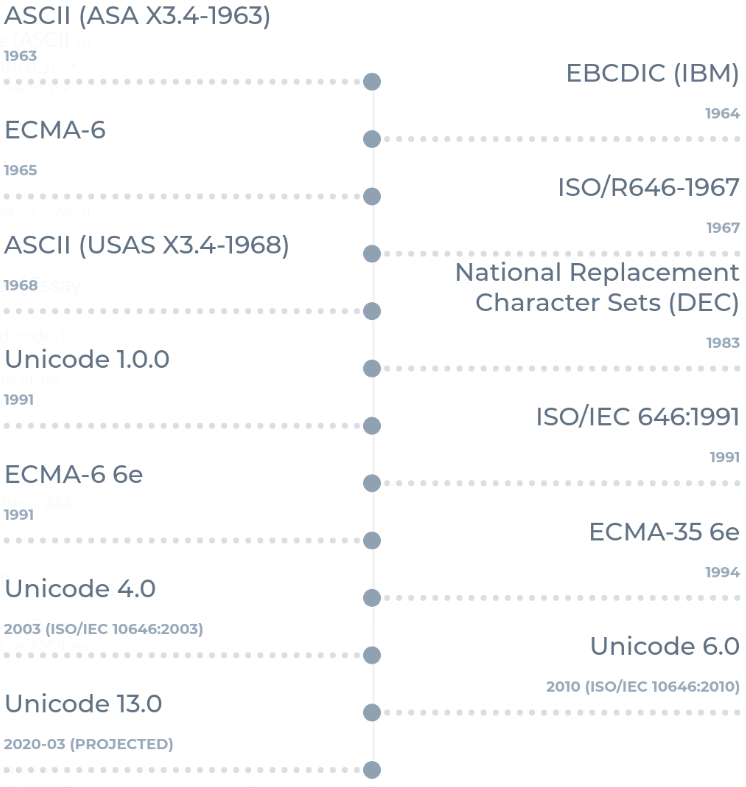
\includegraphics[width=.9\linewidth]{media/charset-timeline.png}
\end{center}


\newpage
%%%%%%%%%%%%%%%%%%%%%%%%%%%%%%%%%%%%%%%%%%%%%%%%%%%%%%%%%%%%%%%%%%%%%%%%
\section{Using ncplanes}
\label{ncplane}
\subsection{Moving and resizing planes}
\subsection{Cells, strings, and formatted output}
\subsection{Alpha blending and plane transparency}
%\newpage

%%%%%%%%%%%%%%%%%%%%%%%%%%%%%%%%%%%%%%%%%%%%%%%%%%%%%%%%%%%%%%%%%%%%%%%%
\section{Styling with colors and attributes}
\subsection{The 32-bit \texttt{attribute} value}
\subsection{The 64-bit \texttt{channels} value}
%\newpage

%%%%%%%%%%%%%%%%%%%%%%%%%%%%%%%%%%%%%%%%%%%%%%%%%%%%%%%%%%%%%%%%%%%%%%%%
\section{Lines, boxes, and fills}
\subsection{Linear interpolation and gradients}
\subsection{Blitting}
%\newpage

%%%%%%%%%%%%%%%%%%%%%%%%%%%%%%%%%%%%%%%%%%%%%%%%%%%%%%%%%%%%%%%%%%%%%%%%
\section{Collecting and dispatching input}
%\newpage

%%%%%%%%%%%%%%%%%%%%%%%%%%%%%%%%%%%%%%%%%%%%%%%%%%%%%%%%%%%%%%%%%%%%%%%%
\section{Multimedia (images and videos)}
\subsection{Scaling images and video}
\subsection{Sprites}
%\newpage

%%%%%%%%%%%%%%%%%%%%%%%%%%%%%%%%%%%%%%%%%%%%%%%%%%%%%%%%%%%%%%%%%%%%%%%%
\section{UI widgets}
\label{section:uiwidgets}
\subsection{Selectors and multiselectors}
\subsection{Menus}
\subsection{Reels}
\subsection{Example: let's rip off \texttt{whiptail}}

\section{Hack the Planet!}
\subsection{Example: let's rip off tetris}
\label{section:casestudy}
\subsection{Example: walking through \texttt{notcurses-demo}}

\newpage
%%%%%%%%%%%%%%%%%%%%%%%%%%%%%%%%%%%%%%%%%%%%%%%%%%%%%%%%%%%%%%%%%%%%%%%%

\begin{appendices}
\section{A brief history of character graphics}
The earliest terminals making use of glyphs\footnote{Konrad Zuse's Z3, generally
 considered the first programmable digital computer, communicated with its
operator through a matrix of blinkenlights and a not unsteampunkish keyboard that resembled the
Burroughs typewriters of its era\cite{zuse}.} printed them to paper, and are of
interest to us only so far as our modern term ``tty'' (of which much will be
said later) is rather dubiously derived from ``TeleTYpewriter'', as these
cantankerous contraptions were known\footnote{Though we do hear of their Snoopy
calendars in the songs of legend\cite{quiche}.} (people had less experience
abbreviating in those days).

These devices most typically printed 72 characters per line (CPL), a limit that
has persisted in strange places\cite{pandoc} through the modern era. Another constant
you'll see from time to time is 132 CPL, derived from line printers such as the
IBM 1403, the DEC LP11, and the Centronics 101\cite{ibm1403}. Most often,
however, is the 80 column line originating in 1928's 7¾x3¼x0.007in IBM
Computer Card (as designed by Clair D.\ Lake, deriving from the 1890 U.\ S.\
Census cards of Herman Hollerith\ldots\ themselves borrowing from Joseph
Jacquard's automation in 1804 of punched card loom control technology pioneered
by Basile Bouchon in 1725\cite{cards}). To this day, so long as your wacky
output device can do 80 columns, eh, that's good enough. In all these cases,
the limit arises from the number of characters that could be printed, using the
technology of the time, on their feeder paper (8.5in and 14in in the case of
printers).

On, then, to the ``Glass TTYs'' (ugh) and Visual Display Units of the 1970s.
Pictured on the next page are the Computer Terminal Corporation Datapoint 3300, the
Lear Sigler, Inc.\ ADM-3A, the Hazeltine 1500, and the Soroc IQ-120.
Lacking microcontrollers, and generally implementing no independent control
sequences, such devices are today often known as ``dumb terminals'' (this term
was originally a registered trademark of Lear Sigler, see below). Already the
80x24 ``standard'' (it is not a standard) was emerging (the DEC contemporaries
listed were already pretty ``smart'', using proprietary control codes):

\vspace{.25in}

\begin{center}
  \begin{tabular}{ |c|c|c| }
    \hline
    IBM 2260 Model 1 & 1965 & 40x6 \\
    \hline
    Datapoint 3300 & 1969 & 72x25 \\
    \hline
    DEC VT05 & 1970 & 72x24 \\
    \hline
    IBM 3277 Model 2 & 1971 & 80x24 \\
    \hline
    Textronix 4010 & 1972 & 74x35 \\
    \hline
    DECscope VT52 & 1974 & 80x24 \\
    \hline
    LSI ADM-3A & 1976 & 80x12, 80x24 \\
    \hline
    Hazeltine 1500 & 1977 & 80x24 \\
    \hline
    Sororc IQ-120 & 1977 & 80x24 \\
    \hline
  \end{tabular}
\end{center}

\vspace{.25in}

The 80 almost certainly arises from the desire to display an entire punched card
(this \textit{is} a standard---see ANSI X3.21-1967/FIPS PUB 13, ``Rectangular
Holes in Twelve-Row Punched Cards'')\cite{sonicdelay}. The origin of 24 is less
clear. 24 is highly composite (it has more divisors than any smaller number),
and it is the largest integer divisible by all natural numbers not larger than its
square root. There are of course 24 hours in a day. 24 divides the scanline
counts of both NTSC and PAL at 480 and 576, respectively. 24 rows of
80 columns at a byte per column utilize 93.75\% of a 2KiB memory, leaving exactly
128 bytes left over, and everyone loves a good power of 2.

The Aaronites, Levite descendents of Moses's brother Aaron, the first
\texthebrew{כהן גדול}
(High Priest),
form the priestly \texthebrew{כֹּהֲנִים}; they were divided into 24 courses. The Buddha's Dharma Chakra (Wheel of Dhamma)
in its Ashoka form extends 24 spokes. But perhaps I grow esoteric, and even
speculative\ldots\ in truth, 80x24 almost certainly owes its questionable
existence to IBM's punched cards, IBM 2260 and 3270 wanting compatibility with
IBM printers, the upstart DEC wanting compatibility with IBM software for their
VT52 and legendary VT100, and the VT100 subsequently becoming a \textit{de facto} standard for
four decades.

\begin{figure}
  \centering
  \begin{minipage}{0.5\textwidth}
    \centering
    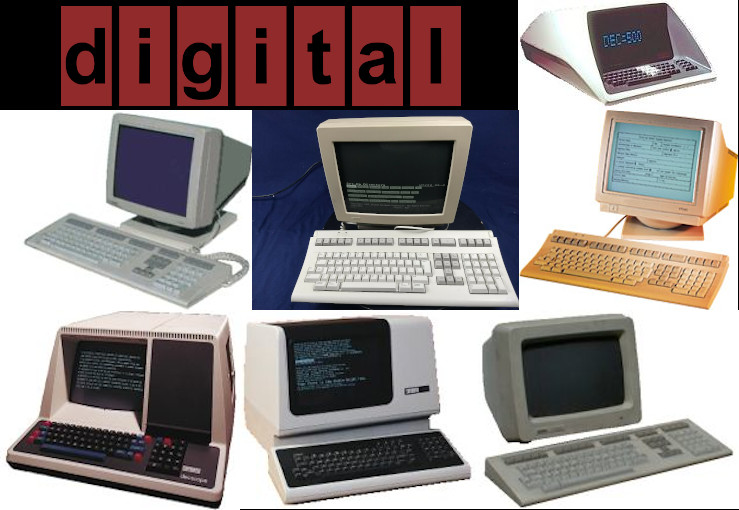
\includegraphics[width=.5\linewidth]{media/digital-terms.jpeg}
    \caption{The Digital Equipment Corporation terminals of the 1970s and 1980s.}
  \end{minipage}\hfill
  \begin{minipage}{0.4\textwidth}
    \centering
    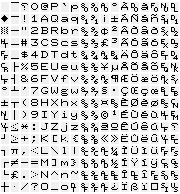
\includegraphics[width=.45\linewidth]{media/vt220-charset.png}
    \caption{The VT220's glyphs from a ROM dump. VT100 implemented most of the
      first seven columns. Note the existence of box-drawing characters\cite{crttypography}.}
  \end{minipage}
\end{figure}

\begin{figure}
  \centering 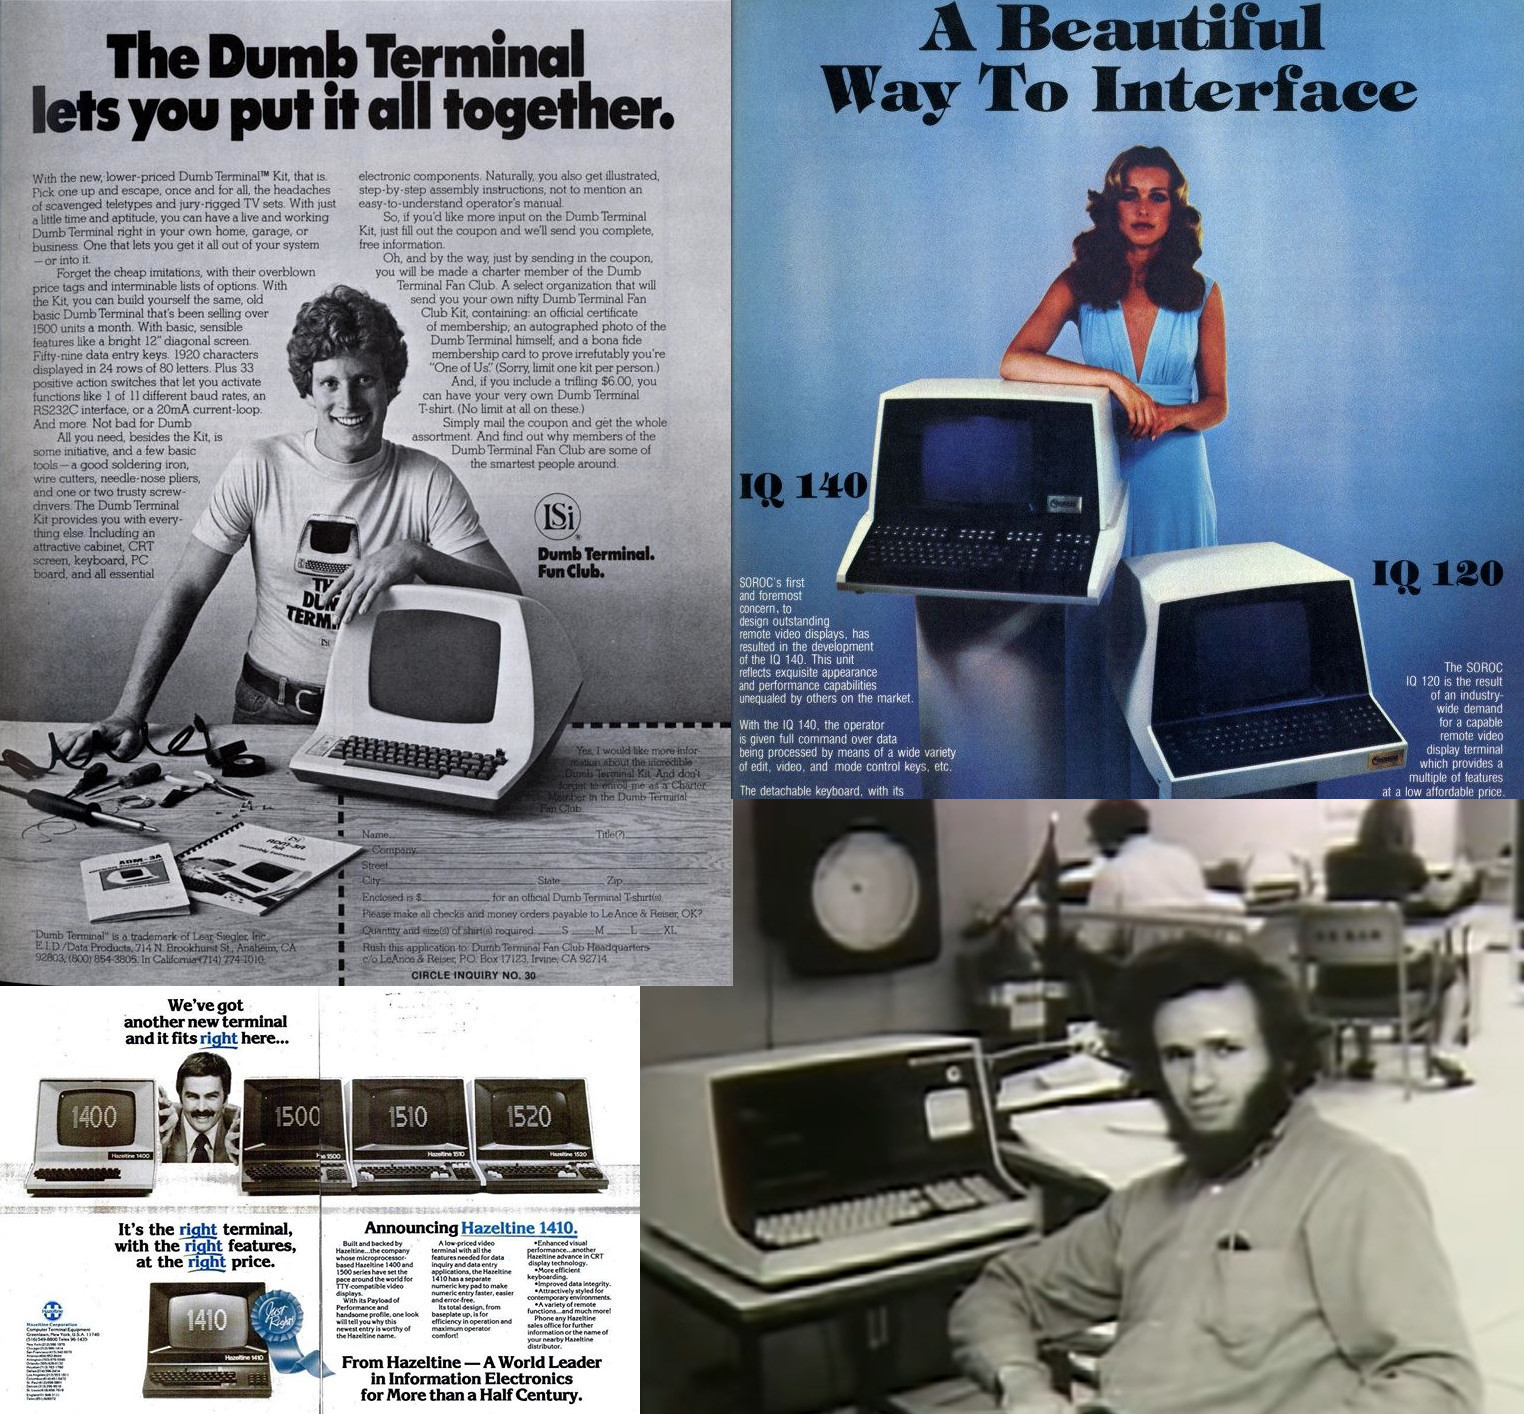
\includegraphics[width=.9\linewidth]{media/dumbterminals.jpg}
\caption{Clockwise starting from upper left: a dork and his LSI ADM (``American
  Dream Machine'', supposedly). That poor woman with the Sororc IQs looks stoned out
  of her gourd. Grizzly Adams rocks a Datapoint 3300, but really his mind is on
  seeing Skynyrd shred it this weekend. Finally, we have Frank the Cocaine
  Ranger and his Electric Hazeltine 1500 Band. \textit{Gott im Himmel}, the 70s were \textit{unseemly}.}
\end{figure}

\subsection{The DEC VTxxx terminals and ANSI X3.64-1979}

Introduced in August 1978, the VT100 ushered in a new era of smart terminals
using commodity (Intel) microprocessors, implementing portions of the upcoming
ANSI X3.64 standard (itself based on 1976's first edition of ECMA-48) along
with DEC extensions\footnote{The VT100 \textit{did not} implement all of X3.64,
nor was X3.64 derived from the VT100. The VT100 didn't do color, nor did it
insert or delete lines. It furthermore implemented several features outside
the scope of ECMA-48's first edition.} This series would go on to sell over
six million units, and it was a rare vendor that didn't include some degree
of DEC VT compatibility. Each major iteration of the series was designed to
encompass all functionality of prior iterations, beginning with the VT100's
faithful emulation of the earlier era's VT52. The VT102 cut down on the cost
and size of the VT100, and included the 132-CPL mode by default; they were
otherwise essentially the same device\cite{vt100}.

The original \texttt{xterm} was written as an emulator of the VAXStation 100
(VS100), and slowly acquired scattered features from the VT100, ANSI, and other
sources\cite{xtermfaq}. Thomas E.\ Dickey (the current maintainer of \Gls{ncurses}
and xterm) began working on XTerm in the mid-90s, and by 1996 had added the
\texttt{decTerminalID} resource following the addition of much VT220 compatibility.

\textbf{FIXME keep goin'\ldots}

\subsection{The Curses API}
\end{appendices}

\newpage
%%%%%%%%%%%%%%%%%%%%%%%%%%%%%%%%%%%%%%%%%%%%%%%%%%%%%%%%%%%%%%%%%%%

\section{The \texttt{notcurses.h} header}
\bgroup
\inputminted[linenos,fontsize=\scriptsize,breaklines=true]{C}{code/notcurses.h}
\egroup
\newpage

%%%%%%%%%%%%%%%%%%%%%%%%%%%%%%%%%%%%%%%%%%%%%%%%%%%%%%%%%%%%%%%%%%%%%%%%
\glsaddallunused
\printglossary[title={Glossary of terms \textit{as used in this manuscript}}]
\newpage
%%%%%%%%%%%%%%%%%%%%%%%%%%%%%%%%%%%%%%%%%%%%%%%%%%%%%%%%%%%%%%%%%%%%%%%%
\addcontentsline{toc}{section}{References}
\printbibliography
%%%%%%%%%%%%%%%%%%%%%%%%%%%%%%%%%%%%%%%%%%%%%%%%%%%%%%%%%%%%%%%%%%%%%%%%
\vfill
\begin{center}

\includegraphics[width=.4\linewidth]{../common/dsscaw-purp-scaled.png}

\includegraphics[width=.5\linewidth]{../common/south.png}
\end{center}
\end{document}
